\chapter{FHE Library Benchmarking}
\chaptermark{FHE Library Benchmarking}
\HRule\\[2cm]
\label{Chapter3}
\lhead{\emph{\textbf{Chapter 3:} FHE Library Benchmarking}}

\begin{spacing}{1.6}

\section{Motivation for Benchmarking}

The choice of FHE library is a foundational decision for any privacy-preserving
ML system. Different libraries expose different parameter configurations,
implement the underlying polynomial arithmetic with different optimisations,
and provide different levels of hardware acceleration. For anomaly detection
specifically, the most critical performance dimensions are:

\begin{itemize}
  \item \textbf{Ciphertext multiplication latency:} Anomaly scoring requires
  at least one ciphertext-ciphertext or ciphertext-plaintext multiplication per
  test observation. For 2000 test rows, even a 10 ms per-operation difference
  accumulates to 20 seconds.
  \item \textbf{Rotation latency:} Computing the sum of $d = 51$ slot values
  requires $\lceil \log_2 51 \rceil = 6$ rotations per row. Rotation is one of
  the most expensive HE operations.
  \item \textbf{Multiplication depth:} The number of sequential multiplications
  possible before the noise budget is exhausted determines which algorithms can
  be implemented without bootstrapping.
  \item \textbf{Noise budget management:} Understanding how quickly noise
  accumulates per operation type is essential for designing depth-efficient
  algorithms.
\end{itemize}

This chapter presents a systematic benchmarking study of three widely used FHE
libraries to characterize these dimensions empirically.

\section{Libraries Under Evaluation}

\subsection{Microsoft SEAL}

Microsoft SEAL \cite{seal} is an open-source C++ FHE library developed by the
Cryptography and Privacy Research Group at Microsoft Research. It implements
the BFV scheme for integer arithmetic and the CKKS scheme for approximate
real valued arithmetic. SEAL is designed for production use, with clean APIs,
extensive documentation, and support for Intel HEXL (Homomorphic Encryption
Acceleration Library), which implements Number Theoretic Transform (NTT)
operations using AVX-512 instructions on compatible Intel processors.

SEAL is accessed from Python via the \texttt{seal-python} wrapper, which
provides bindings to all major SEAL operations with minimal overhead relative
to the C++ implementation.

\subsection{IBM HElib}

IBM HElib \cite{helib} is an open-source C++ FHE library developed by IBM
Research. It implements the BGV scheme and a variant of CKKS, and is the only
library in this study that supports bootstrapping --- the operation that
refreshes the noise budget to enable computation of circuits deeper than the
initial level budget. HElib is a research-oriented library with support for
advanced features but a steeper learning curve than SEAL.

\subsection{Pyfhel}

Pyfhel \cite{pyfhel} is a Python-native FHE library that provides a simplified
interface to SEAL and HElib operations. Its primary advantage is accessibility:
it requires no C++ knowledge and provides intuitive Python syntax. However, it
does not support Intel HEXL acceleration, and its abstraction layer introduces
overhead relative to direct SEAL usage. Pyfhel is best suited for rapid
prototyping and educational purposes.

\section{Experimental Methodology}

\subsection{Parameter Configurations}

To ensure a fair and unbiased comparison, all experiments used a unified set
of parameter configurations:

\begin{itemize}
  \item \textbf{Polynomial modulus degrees:} 1024, 4096, 8192, 16384, 32768
  \item \textbf{Coefficient modulus chains:} Default chains provided by each
  library for each polynomial degree
  \item \textbf{Vector sizes:} 16, 64, 256, 1024, 4096, 16384, 65536, 1,048,576
  \item \textbf{Data distributions:} Constant (same integer in all slots) and
  Random (uniformly random integers)
  \item \textbf{Repetitions:} 10 independent runs per configuration, results
  averaged to reduce timing variability
\end{itemize}

This methodology ensures that observed performance differences arise from
library implementation characteristics rather than parameter inconsistencies.

\subsection{Experiment 1: Arithmetic Operation Latency}

This experiment measures encryption time, decryption time, and operation latency
for the four core homomorphic arithmetic operations:
\begin{itemize}
  \item Ciphertext + Ciphertext (ct+ct)
  \item Ciphertext + Plaintext (ct+pt)
  \item Ciphertext $\times$ Plaintext (ct$\times$pt)
  \item Ciphertext $\times$ Ciphertext (ct$\times$ct)
\end{itemize}

Each operation was benchmarked with and without Intel HEXL acceleration (where
supported) and across both data distributions.

\subsection{Experiment 2: Rotation Operation Latency}

Rotations are one of the most expensive operations in HE because they require
key-switching using precomputed Galois keys. Three rotation types were measured:
left rotation (shift slots left by one position), right rotation (shift right),
and column rotation (Galois automorphism that swaps the two halves of the slot
vector). Timings were collected across all polynomial degrees and vector sizes.

\subsection{Experiment 3: Maximum Operation Depth}

This experiment determines the maximum number of successive operations of each
type before noise budget exhaustion causes decryption to produce incorrect
results. For multiplicative operations (ct$\times$ct, ct$\times$pt), this
corresponds directly to the number of available levels. For additive operations,
the noise growth per operation is much smaller, enabling a much larger number
of operations.

\subsection{Experiment 4: Noise Budget Evolution}

This experiment tracks the remaining noise budget after applying operations in
increasing powers of two (1, 2, 4, 8, 16, ...) operations, providing insight
into the rate of noise accumulation per operation type. This analysis motivates
the algorithm design principle of minimising multiplicative depth.

\section{Results: Experiment 1 --- Arithmetic Operations}

\subsection{SEAL Results}

\textbf{Encryption and Decryption:} Encryption times range from 1.1--1.7 ms
at degree 4096 to 13.4--57.1 ms at degree 32768, with HEXL providing consistent
8--15\% improvement. Decryption is consistently faster than encryption for the
same parameters, with 5--12\% HEXL speedup.

\textbf{Ciphertext-Ciphertext Addition (ct+ct):} Performance is largely
insensitive to vector size for fixed polynomial degree, ranging from 0.011--0.08
ms at degree 4096. HEXL provides 10--25\% acceleration, with larger benefits
at higher polynomial degrees. Same-data vectors are 15--35\% faster than random.

\textbf{Ciphertext-Plaintext Addition (ct+pt):} Similar to ct+ct but slightly
faster (0.075--0.15 ms at degree 4096), with 8--20\% HEXL improvement.

\textbf{Ciphertext-Plaintext Multiplication (ct$\times$pt):}
Substantially more expensive than addition (8--10$\times$), ranging from
0.057--40.42 ms. HEXL provides significant 15--35\% acceleration, with
larger polynomial degrees benefiting most.

\textbf{Ciphertext-Ciphertext Multiplication (ct$\times$ct):}
The most computationally expensive operation, ranging from 3.37--439.42 ms.
This is 50--100$\times$ more costly than ct+ct and 5--10$\times$ more costly
than ct$\times$pt. HEXL provides the maximum benefit here: 20--45\%
improvement, with the highest gains at degree 32768.

\subsection{HElib Results}

HElib's arithmetic performance is substantially weaker than SEAL for most
operation types. The most notable anomaly is ct$\times$pt, which is
approximately 80--100$\times$ more expensive than addition operations in
HElib (versus 8--10$\times$ in SEAL), making it a poor choice for algorithms
that multiply ciphertexts by plaintext vectors. HElib's ct$\times$ct
performance is comparable to or slower than SEAL at the same polynomial degree,
with inconsistent HEXL benefits.

\subsection{Pyfhel Results}

Pyfhel shows stable ct$\times$ct performance (3.51--8.09 ms at degree 4096)
but a significant performance anomaly in ct$\times$pt for same-data vectors,
which can be 60--90\% faster than random-data vectors. This suggests Pyfhel
applies a constant-factor optimization for repeated-value plaintexts. The
absence of HEXL support means Pyfhel consistently underperforms SEAL for all
operations at larger polynomial degrees.

\begin{table}[H]
\centering
\caption{Arithmetic Operation Latency Comparison at Degree 4096 (ms)}
\label{tab:arith}
\begin{tabular}{lcccc}
\toprule
\textbf{Operation} & \textbf{SEAL} & \textbf{SEAL+HEXL} & \textbf{HElib} & \textbf{Pyfhel} \\
\midrule
Encryption & 1.1--1.7 & 0.95--1.5 & 4.66--5.86 & 1.33--3.57 \\
Decryption & 0.31--0.66 & 0.28--0.60 & 0.91--46.70 & 0.36--0.57 \\
ct+ct & 0.011--0.08 & 0.009--0.06 & 0.022--0.08 & 0.038--0.18 \\
ct+pt & 0.075--0.15 & 0.062--0.12 & 0.023--0.09 & 0.078--0.14 \\
ct$\times$pt & 0.057--0.40 & 0.040--0.28 & 3.44--8.0 & 0.037--1.22 \\
ct$\times$ct & 3.37--4.20 & 2.10--3.30 & 3.44--50.0 & 3.51--8.09 \\
\bottomrule
\end{tabular}
\end{table}

\section{Results: Experiment 2 --- Rotation Operations}

\subsection{SEAL Rotation Performance}

Left rotation exhibits super-linear scaling with polynomial degree in SEAL:
from 0.83 ms at degree 4096 to 4698.58 ms at degree 32768. HEXL provides
10--60\% reduction in rotation time, with the largest gains at the highest
polynomial degrees. Right rotation performs similarly to left rotation.
Column rotation also exhibits similar cost to single-position rotations.

\subsection{HElib Rotation Performance}

HElib shows more favourable (approximately linear) scaling with polynomial
degree for rotations: from 7.96 ms at degree 4096 to 85.56 ms at degree 32768
(approximately 10$\times$ increase versus SEAL's 500$+$ $\times$ increase).
A notable characteristic is that column rotation in HElib is 2--4$\times$
faster than single-position rotations, indicating a highly optimised Galois
automorphism implementation. Right rotations are consistently 1.5--1.8$\times$
slower than left rotations.

\subsection{Pyfhel Rotation Performance}

Pyfhel rotation scales similarly to SEAL (super-linear) but is faster at the
lowest polynomial degrees. Column rotation degrades significantly at large vector
sizes, being 2--3$\times$ slower than single-position rotations.

\begin{table}[H]
\centering
\caption{Left Rotation Latency Across Polynomial Degrees (ms)}
\label{tab:rotation}
\begin{tabular}{lcccc}
\toprule
\textbf{Library} & \textbf{4096} & \textbf{8192} & \textbf{16384} & \textbf{32768} \\
\midrule
SEAL (no HEXL) & 0.83 & 4.1 & 26 & 4698 \\
SEAL (HEXL) & 0.70 & 3.1 & 16 & 160$+$ \\
HElib & 7.96 & 17--34 & 36--66 & 75--137 \\
Pyfhel & 0.76 & 3.7--11.6 & 23.3--70.5 & 143.3--436.4 \\
\bottomrule
\end{tabular}
\end{table}

At the working polynomial degree of 16384, SEAL with HEXL achieves 16 ms per
rotation, which for 6 rotations per row amounts to approximately 96 ms per
test row for the slot-sum operation alone. This is acceptable for a batch of
2000 test rows.

\section{Results: Experiment 3 --- Maximum Operation Depth}

\textbf{Addition operations:} All libraries support over 1,048,576 successive
addition operations before decryption failure, as the noise contribution per
addition is negligibly small. In practice, the number of useful additions approximately is
unlimited for the purposes of anomaly detection algorithms.

\textbf{Multiplication operations:} Depth is severely constrained and increases
with polynomial degree, as larger degrees allow longer modulus chains:

\begin{table}[H]
\centering
\caption{Maximum ct$\times$ct Operations Before Decryption Failure}
\label{tab:depth}
\begin{tabular}{lcccc}
\toprule
\textbf{Library} & \textbf{Deg.\ 4096} & \textbf{Deg.\ 8192} & \textbf{Deg.\ 16384} & \textbf{Deg.\ 32768} \\
\midrule
SEAL & 9 & 14 & 23 & 32 \\
HElib & 7 & 12 & 19 & 27 \\
Pyfhel & 5 & 9 & 14 & 19 \\
\bottomrule
\end{tabular}
\end{table}

At the working degree of 16384, SEAL supports 23 levels, more than sufficient
for both HE-SAD (2 levels per row) and HE-PCA (3 levels per row) with a custom
modulus chain of $[60,40,40,40,40,40,60]$ configured for exactly 5 usable
levels.

\section{Results: Experiment 4 --- Noise Budget Evolution}

The noise budget experiment reveals a fundamental asymmetry between addition
and multiplication:

\textbf{Addition:} Noise growth per addition is negligible --- after
1,048,576 successive additions, the noise budget had decreased by less than
0.1\% of its initial value. This validates the use of rotation-and-add
sequences for slot summation, as 6 rotations plus 6 additions contribute
negligible noise.

\textbf{Multiplication:} Each ciphertext$\times$ciphertext multiplication
consumes approximately $1/L$ of the remaining noise budget at polynomial degree
32768, where $L$ is the total number of primes in the modulus chain. This rapid
depletion directly motivates the algorithm design principle: minimize
multiplications, not additions, in anomaly scoring formulas.

This result directly informs the algorithm design in Chapter~4 and Chapter~5:
every multiplication in the anomaly scoring formula must be justified, and
additions (including the 6 rotations for slot sums) are essentially free.

\section{Library Selection Decision}

Based on the four experiments, Microsoft SEAL is selected as the implementation
foundation for the privacy-preserving anomaly detection system.

\begin{table}[H]
\centering
\caption{Comprehensive Library Comparison Summary}
\label{tab:libsummary}
\begin{tabular}{p{4cm}p{3cm}p{3cm}p{3cm}}
\toprule
\textbf{Criterion} & \textbf{SEAL} & \textbf{HElib} & \textbf{Pyfhel} \\
\midrule
ct$\times$ct speed (4096) & Best (4.2 ms) & Worst (3.44--50 ms) & Medium (3.51--8 ms) \\
ct$\times$pt speed & Best & Worst (80--100$\times$ addition) & Good \\
HEXL acceleration & Consistent 15--45\% & Inconsistent & Not supported \\
Rotation scaling & Super-linear & Linear (better) & Super-linear \\
Max depth (deg.\ 32768) & 32 (best) & 27 & 19 (worst) \\
Bootstrapping & No & Yes (unique) & No \\
Python API & Via wrapper & Via wrapper & Native \\
Documentation & Excellent & Good & Good \\
\bottomrule
\end{tabular}
\end{table}

The rationale for selecting SEAL:

\begin{enumerate}
  \item \textbf{Best ct$\times$ct performance:} Anomaly scoring requires at
  least one multiplication per test row. At 2000 test rows, SEAL's 4.2 ms
  versus HElib's up to 50 ms represents a substantial throughput advantage.

  \item \textbf{Superior ct$\times$pt performance:} Both HE-SAD
  (multiplication by $1/\sigma^2$) and HE-PCA (projection onto component
  vectors) rely heavily on ct$\times$pt operations. HElib's anomalously
  expensive ct$\times$pt makes it impractical for these algorithms.

  \item \textbf{Deepest multiplication budget:} SEAL achieves depth 32 at
  degree 32768, providing the most headroom for complex algorithms, and at the
  working degree of 16384 supports 5 configurable levels --- sufficient for
  both detection algorithms.

  \item \textbf{Consistent HEXL acceleration:} SEAL's HEXL integration provides
  reliable 15--45\% speedup for all operation types, particularly benefiting
  the rotation-heavy slot-sum operations in anomaly scoring.
\end{enumerate}

HElib would be preferred in scenarios requiring bootstrapping (circuits deeper
than the initial level budget). Pyfhel would be preferred for educational
purposes or initial prototyping. For production anomaly detection, SEAL is the
clear choice.

\section{Benchmarking Result Plots}

The following figures present the empirical results from all four benchmarking
experiments, visualising the performance characteristics discussed in the
preceding sections.

\end{spacing}

\begin{figure}[!ht]
\centering
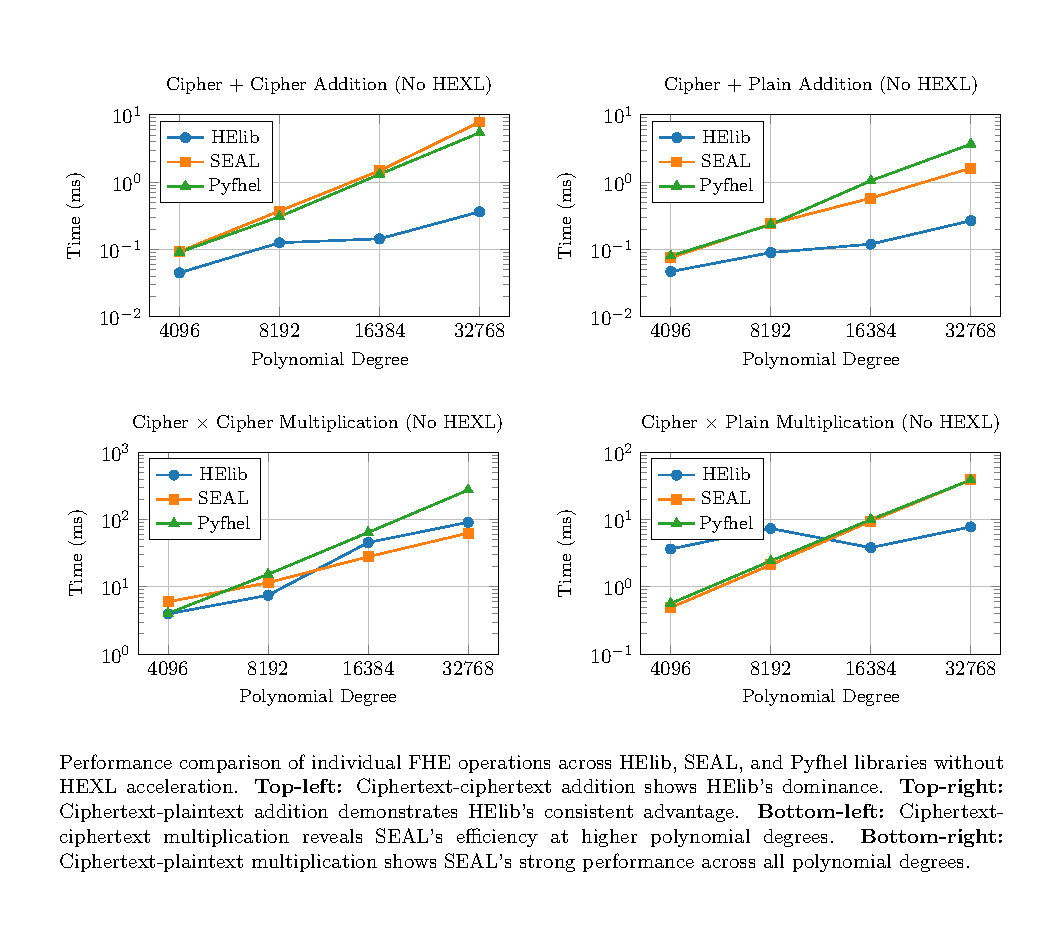
\includegraphics[width=\textwidth]{Images/atithematic_plot.pdf}
\caption{Experiment 1: Arithmetic Operation Latency Comparison Across SEAL,
HElib, and Pyfhel at Polynomial Degree 4096, with and without Intel HEXL
acceleration.}
\label{fig:exp1_arith}
\end{figure}

\begin{figure}[!ht]
\centering
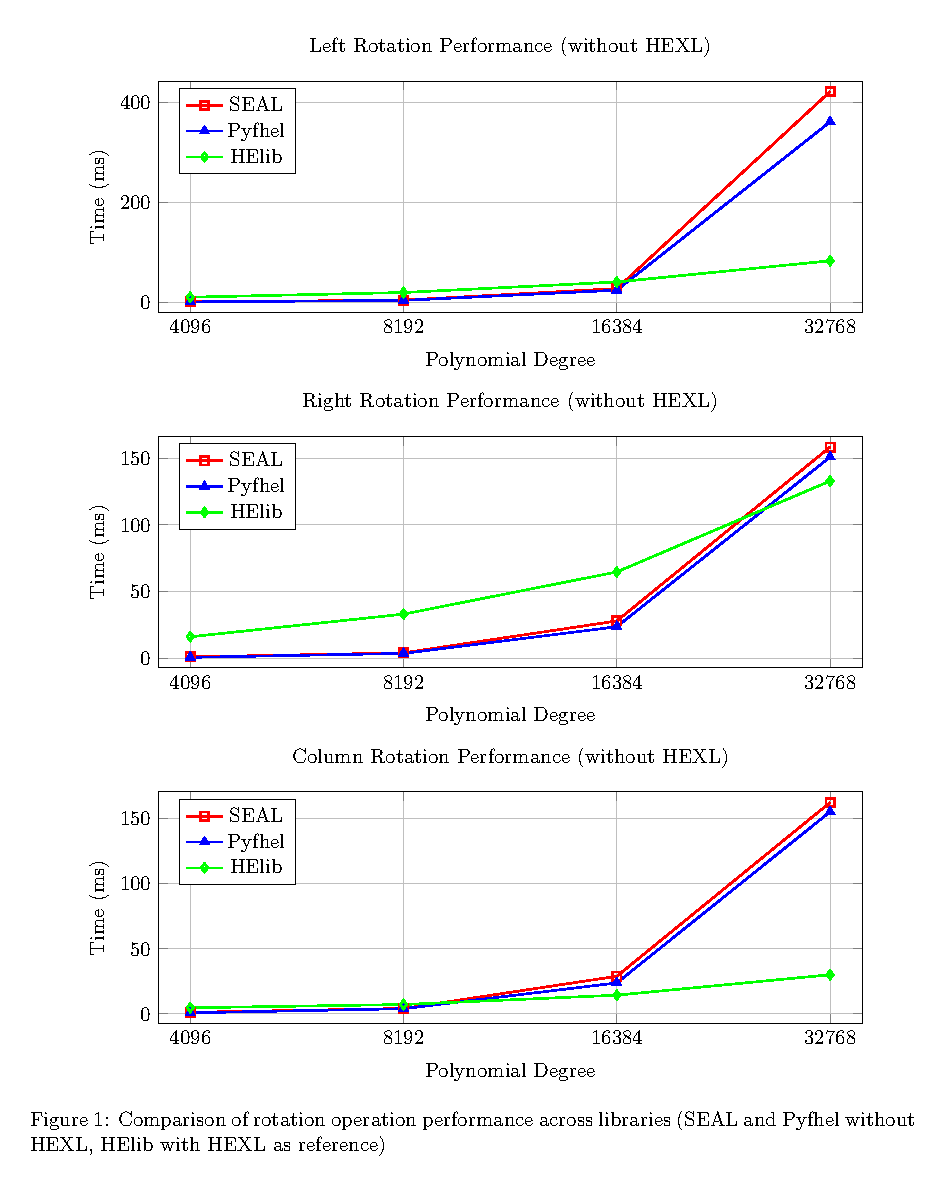
\includegraphics[width=\textwidth]{Images/rotation_comparison (2).pdf}
\caption{Experiment 2: Left Rotation Latency Scaling with Polynomial Degree
Across Libraries. SEAL exhibits super-linear scaling while HElib scales
approximately linearly.}
\label{fig:exp2_rotation}
\end{figure}

\begin{figure}[!ht]
\centering
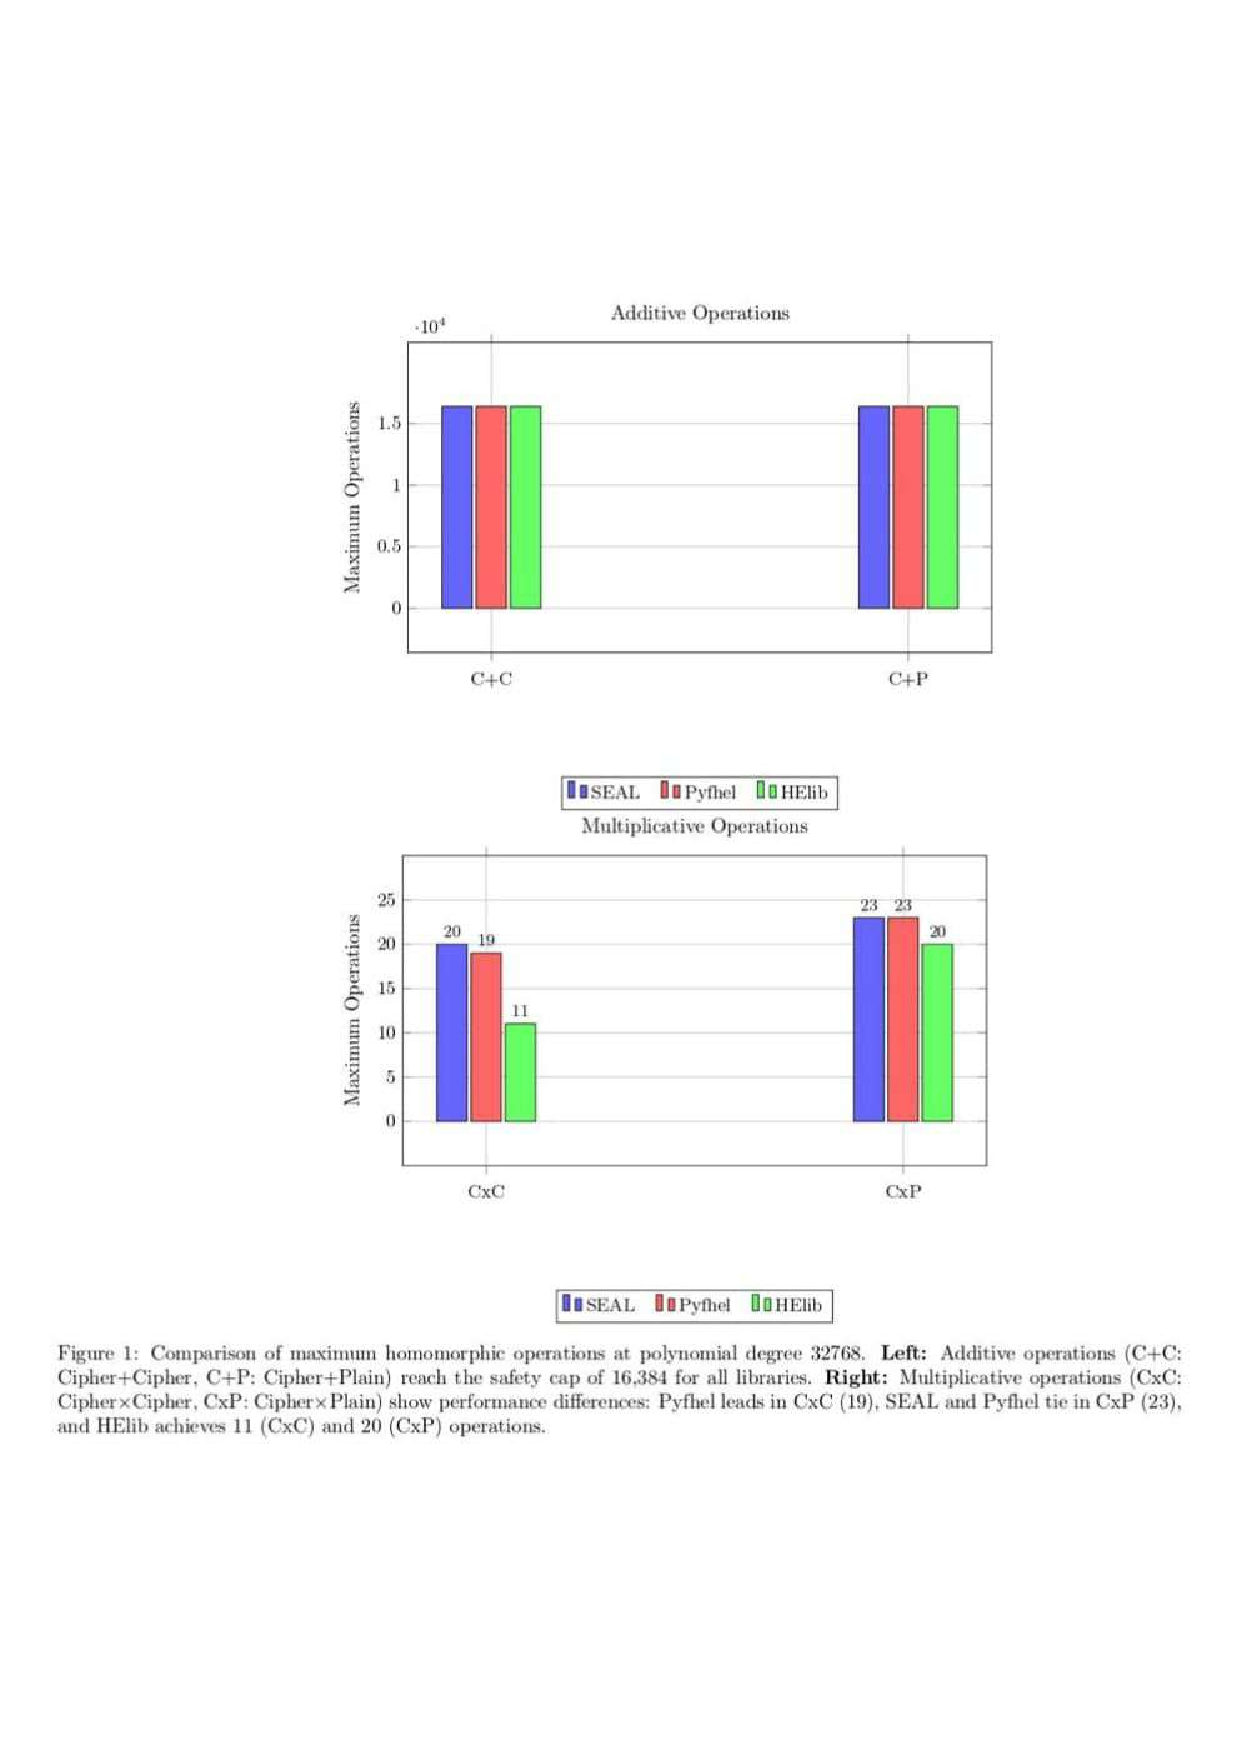
\includegraphics[width=\textwidth]{Images/depth_analysis.pdf}
\caption{Experiment 3: Maximum ct$\times$ct Multiplication Depth Before
Decryption Failure. SEAL achieves the deepest multiplication budget at all
polynomial degrees.}
\label{fig:exp3_depth}
\end{figure}

\begin{figure}[!ht]
\centering
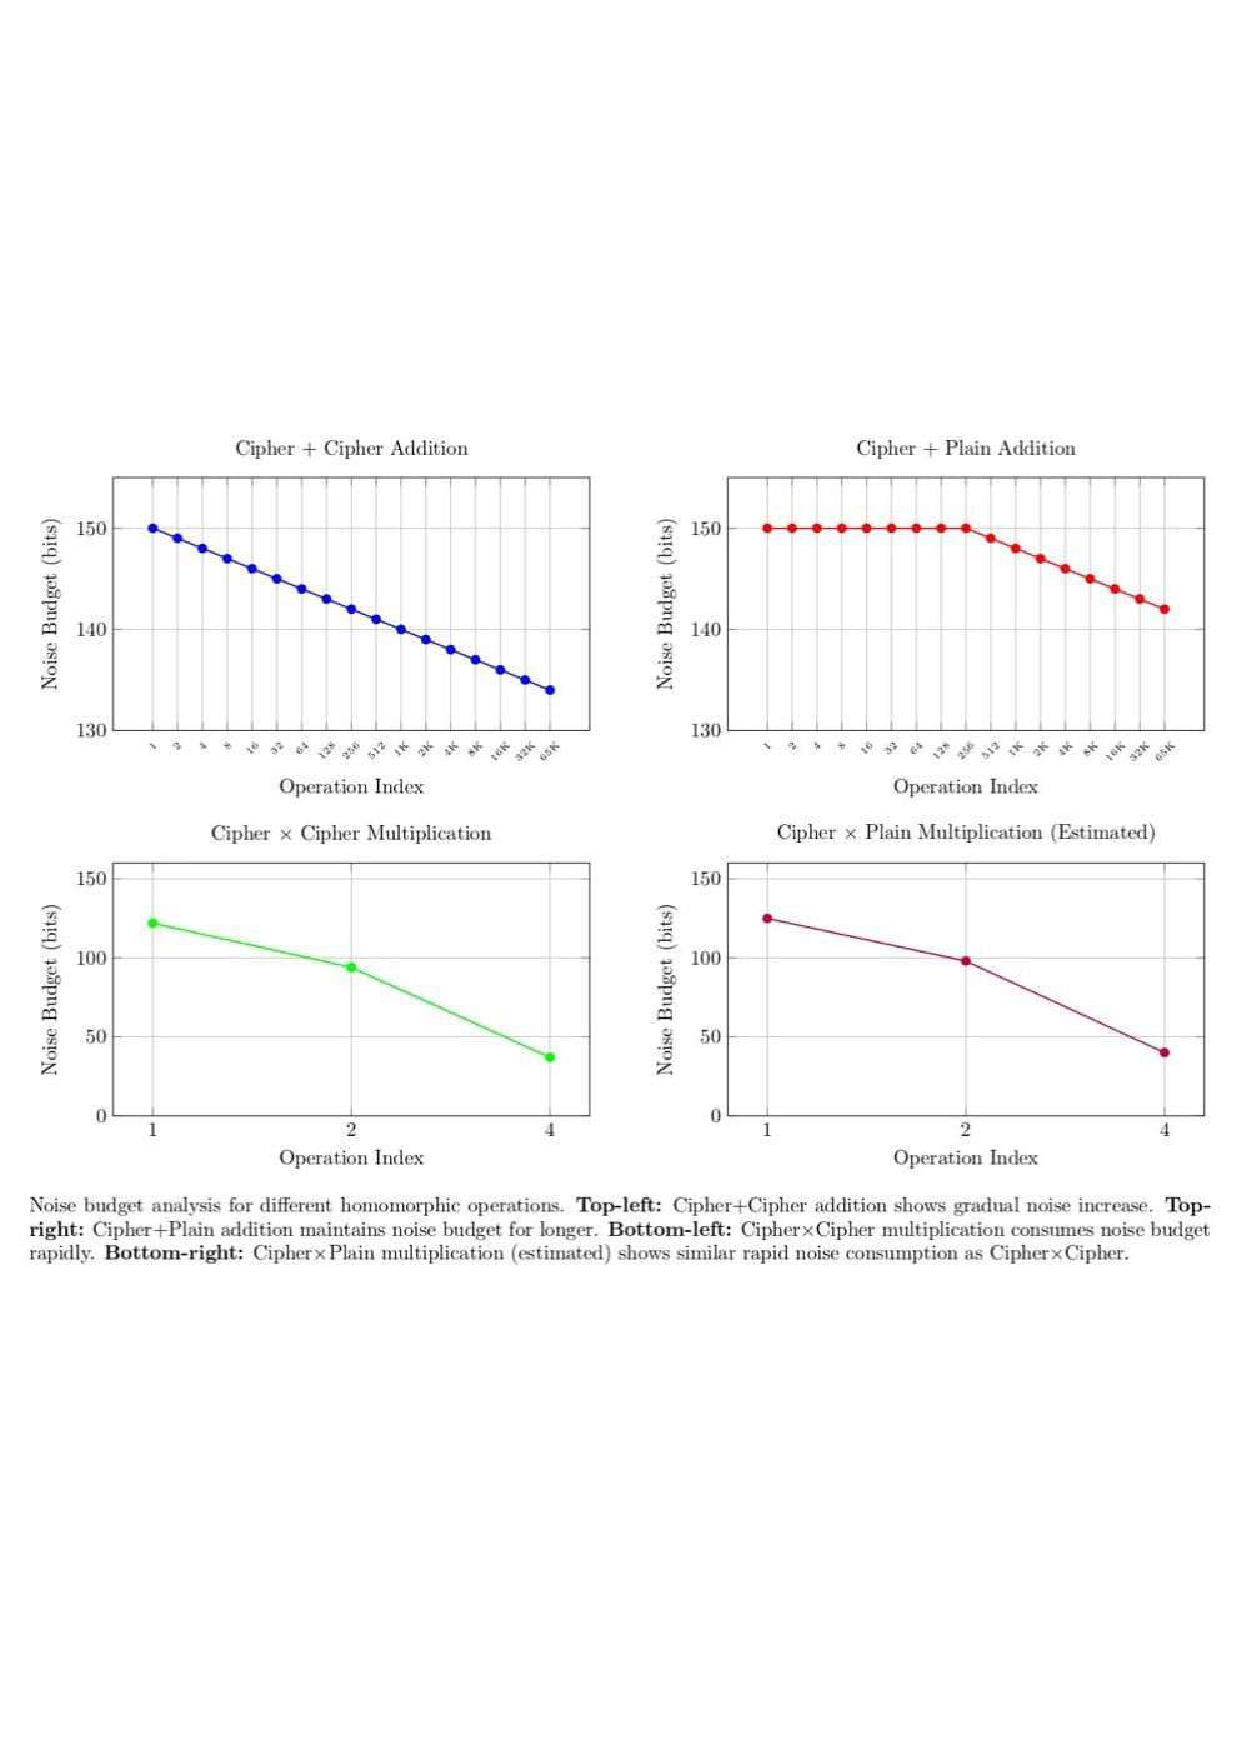
\includegraphics[width=\textwidth]{Images/noise_analysis.pdf}
\caption{Experiment 4: Noise Budget Evolution with Successive Multiplication
Operations. Each multiplication consumes approximately $1/L$ of the remaining
budget, directly motivating depth-efficient algorithm design.}
\label{fig:exp4_noise}
\end{figure}